\documentclass[11pt]{article}
\usepackage[utf8]{inputenc}
\usepackage{color}
\usepackage{amsmath}
\usepackage{algorithm}
\usepackage{algorithmic}
\usepackage{subfiles}
\usepackage{titling}
\usepackage{geometry}
\usepackage{graphicx}
\usepackage{xspace}
\usepackage{docmute}
\usepackage{lipsum}
\usepackage{makecell}
\usepackage{ragged2e}
\usepackage{multirow}
\usepackage{paralist}
\usepackage[dvipsnames]{xcolor}
\fboxsep0pt

\usepackage{caption}
\usepackage{glossaries}

\usepackage{hyperref}
\hypersetup{
  colorlinks=true,
  linkcolor=blue,
  filecolor=magenta,      
  urlcolor=cyan,
  pdftitle={This test},
  pdfpagemode=FullScreen,
}
\urlstyle{same}

\DeclareUnicodeCharacter{2212}{-}


\renewcommand{\labelenumii}{\arabic{enumi}.\arabic{enumii}}
\usepackage[inline]{enumitem}
\newcommand{\METRICSTICS}{\texttt{METRICSTICS}\xspace}
\begin{document}

\begin{figure}
    \centering
    
\includegraphics[width=14cm]{Concordia-logo.jpeg}
    \label{fig:Concordia}
\end{figure}

\title{SOEN 6611 \\ \vspace{\baselineskip}  DELIVERY 2 \\ Team J}
\author{%
  Quoc Phong Ngo \\
  SanVinoth Pacham   \\
  Preet Angad Singh  \\
  Siddharth Bharat Oza   \\
  Nomesh Palakaluri
}



\maketitle

\centering{\href{https://github.com/Nomesh88/SOEN6611/tree/main}{Github Link}}
\pagebreak
\tableofcontents

\pagebreak

\section*{Symbols and Abbreviations}

\begin{table}[htb]
    \centering
    \begin{tabular}{|p{2cm}|p{7.5cm}|} \hline 
         GQM & Goal Metric Question \\ \hline
         UC & Use Case \\ \hline
         HRM & Human Resource Management \\ \hline
         SLOC & Source Line of Codes SLOC(L) Logical SLOC \\ \hline
         UCP & Use Case Point \\ \hline
         PF & Productivity Factor \\ \hline
         UUCP & Unadjusted Use Case Points \\ \hline
         TCF & Technical Complexity Factor \\ \hline
         Ecf & Environmental Complexity Factor \\ \hline
         UAW & Unadjusted Actor Weight \\ \hline
         UUCW & Unadjusted Use Case Weight \\ \hline
         WTi & Technical Complexity Factor Weight \\ \hline
         Fi & Perceived Impact Weight \\ \hline
         WEi & Environmental Complexity Factor Weight \\ \hline
    \end{tabular}
    \label{tab:my_label}
\end{table}

\section*{List of Figures}
\normalsize{
\raggedright{
\hyperref[sec: Use Case Diagram]{3.1 METRICSTICS Application}. . . . . . . . . . . . . . . .  . . . . . . . . .  . . . . . . . 11 \\
\hyperref[sec: Use Case Diagram]{3.2 Code Sample} . . . . . . . . . . . . . . . . . . . . . . . . .  . . . . . . . . .  . . . . . . . 12 \\
\hyperref[sec: Use Case Diagram]{3.3 Python Structure Classes}. . . . . . . . . . . . . . . . . .  . . . . . . . . .  . . . . . . . 13 \\
\hyperref[sec: Use Case Diagram]{4.1 Cyclometric Complexity of Metristics clas} . . . . . . . .  . . . . . . . . . . . . . . . . 16\\
\hyperref[sec: Use Case Diagram]{4.2 Cyclometric Complexity of MetristicsFrame class}. . . .  . . . . . . . . .  . . . . . . . 16\\
\hyperref[sec: Use Case Diagram]{4.3 Cyclometric Complexity of DataGenerator class} . . . . . . . .  . . . . . . . . .  . . . 17\\
\hyperref[sec: Use Case Diagram]{4.4 Cyclometric Complexity of LoginWindow clas}. . . . . . . . . . . . . . .  . . . . . . . 17\\
\hyperref[sec: Use Case Diagram]{4.5 Cyclometric Complexity of App class} . . . . . . . . . . . . . . . . . . . . .  . . . . . . 17\\
\hyperref[sec: Use Case Diagram]{5.1 Overall dependencies of the System}. . . . . . . . . . . .  . . . . . . . . .  . . . . . . . .24\\
\hyperref[sec: Use Case Diagram]{6.1 Physical and Logical SLOC} . . . . . . . . . . . . . . . . . . . . . . . . . . .  . . . . . . 26\\
}}

\pagebreak
\section{Background Information}
\raggedright{\normalsize{The development of the Healthcare Workers Analytics Platform, referred to as METRICSTICS, will entail the creation of a pivotal system aimed at providing a holistic analysis of healthcare workforce performance. This system is envisioned to conduct robust statistical examinations of various workforce metrics, thus equipping healthcare management with valuable tools to effectively oversee trends in staffing and optimize workforce strategies. Access to METRICSTICS will be extended to healthcare personnel, including both frontline healthcare workers and administrative staff, fostering collaborative data input processes for the former and seamless access to statistical insights for the latter. Furthermore, METRICSTICS will facilitate the generation of comprehensive reports, which will be presented periodically to the governing board, offering critical insights for informed decision-making.}} \\[2\baselineskip]
\raggedright{\normalsize{Remark: The primary stakeholders for METRICSTICS encompass healthcare workers, including frontline staff and administrative personnel, as well as healthcare management and governing authorities.}}

\pagebreak
\section{Problem 3: Use Case Points(UCP)}

\subsection{Using the use case points (UCP) approach (or one of its extensions), provide an estimate of the effort towards the project. }

\subsubsection{Introduction}
\normalsize{The relationship between use cases and effort in software development is that use cases help define the functional requirements of a system and serve as a basis for estimating the effort (time, resources) required to develop the software. The complexity and granularity of use cases can influence the accuracy of effort estimation, and they also assist in prioritizing tasks, communication, and risk management throughout the project.}

\subsubsection{Effort Estimate using Use Case Point approach}
\normalsize{These are a few steps required for the effort estimation process\\
1. Determine and Calculate Unadjusted Use Case Points (UUCP).\\
2. Determine and Calculate Technical Complexity Factor (TCF).\\
3. Determine and Calculate Environment Complexity Factor (ECF).\\
4. Determine Productivity Factor (PF).\\
5. Calculate Use Case Points (UCP).\\
6. Calculate the Estimated Number of Person-Hours. \linebreak \\

\normalsize{The \textbf{effort estimate} is determined by multiplying the Use Case Points by the Productivity Factor.}

\normalsize{\centerline{Effort Estimate = UCP * PF (3.1) }}
\hfill\break
\normalsize{The \textbf{UCP} equation can be expressed as follows:}

\normalsize{\centerline{UCP = UUCP * TCF * ECF (3.2) \linebreak[2]}}
\hfill\break
\normalsize{\textbf{UUCP} is determined by adding the Unadjusted Actor Weight (UAW), reflecting actor complexity, and the Unadjusted Use Case Weight (UUCW), representing the total scenario steps. \linebreak}

\normalsize{The formula for UUCP is:}
\normalsize{\centerline{UUCP = UAW + UUCW (3.3) \linebreak}}
\hfill\break

\normalsize{The Unified Function Point (UCP) calculation recognizes that not all actors in a use case model are equal in terms of complexity. There are three types of actors:}

\begin{inparaitem}
    \item Simple Actor
    \item Average Actor
    \item Complex Actor
\end{inparaitem}

\normalsize{In summary, a simple actor is a machine, an average actor can be either a human or a machine, and a complex actor is a human. These distinctions help in assessing actor complexity in UCP calculations. \linebreak}

\normalsize{In our use case model, we have a single actor, the user, who interacts with the system through a graphical user interface. Consequently, this actor is classified as a \textbf{complex actor}, and it is assigned a weight of 3 points, resulting in:}

\normalsize{\centerline{UAW = 3}}
\hfill\break

\normalsize{We have x classes in the system.so, it comes under average use case.}
\centerline{UUCW=10}
\normalsize{From 3.3:}
\normalsize{\centerline{UUCP=UAW + UUCW}
\centerline{UUCP = 3 + 10}
\centerline{UUCP = 13}
\hfill\break

\normalsize{\textbf{TCF} is a multiplier that assesses the impact of technical and environmental factors on a software project's complexity. It's used to adjust function points and estimate development effort, aiding in project planning. It consists of 13 different factors, each with there own weight.}


\label{sec: Figure 6}
\begin{figure}[htp]
    \centering
    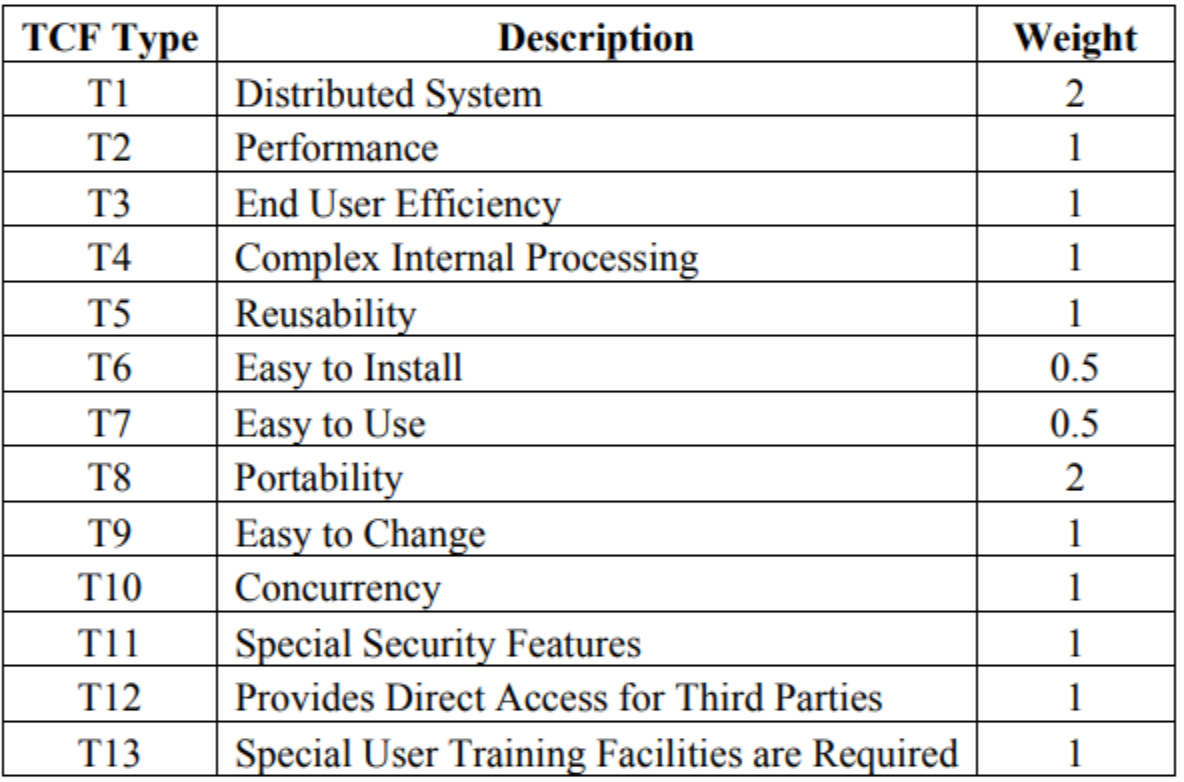
\includegraphics[width=15cm, height=9cm]{p6.png}
    \label{fig:Figure 6}
    \descriptionlabel{Table 2.1 The Technical Complexity Factors in the UCP approach.}
\end{figure}

\pagebreak

\normalsize{The equation is given by:}

\label{sec: Figure 7}
\begin{figure}[htp]
    \centering
    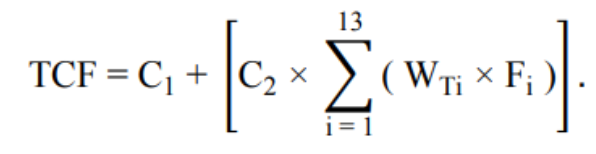
\includegraphics[width=8cm, height=2cm]{p7.png}
    \label{fig:Figure 7}
\end{figure}

\normalsize{C1=0.6 and C2=0.01, WTi is Technical Complexity Factor Weight, Fi is Perceived Impact Factor. \linebreak \\
Fi is decided based on the values of:\\}
\begin{inparaitem}
    \item No influence = 0
    \item Average influence = 3
    \item Strong influence = 5 \linebreak \\
\end{inparaitem}

\normalsize{In our case,}
\begin{itemize}[noitemsep]
    \item No Influence - T1,T10,T11,T12,T13
    \item Average Influence - T2,T3,T4
    \item Strong Influence - T5,T6,T7,T8,T9
\end{itemize}

{\normalsize{TCF=0.6+(0.01*((2*0)+(1*3)+(1*3)+(1*3)+(1*5)+(0.5*5)+(0.5*5)+(2*5)+(1*5)+(1*0)+
(1*0)+(1*0)+(1*0)))\linebreak}
\normalsize{TCF = 0.6 + (0.01*44)\linebreak}
\normalsize{TCF = 1.04 \linebreak \\}

\normalsize{The Environmental Complexity Factor (\textbf{ECF}) is a multiplier that quantifies how external and environmental factors affect the complexity of a software project. It's used to adjust function points and estimate development effort, facilitating project planning.
}

\label{sec: Figure 8}
\begin{figure}[htp]
    \centering
    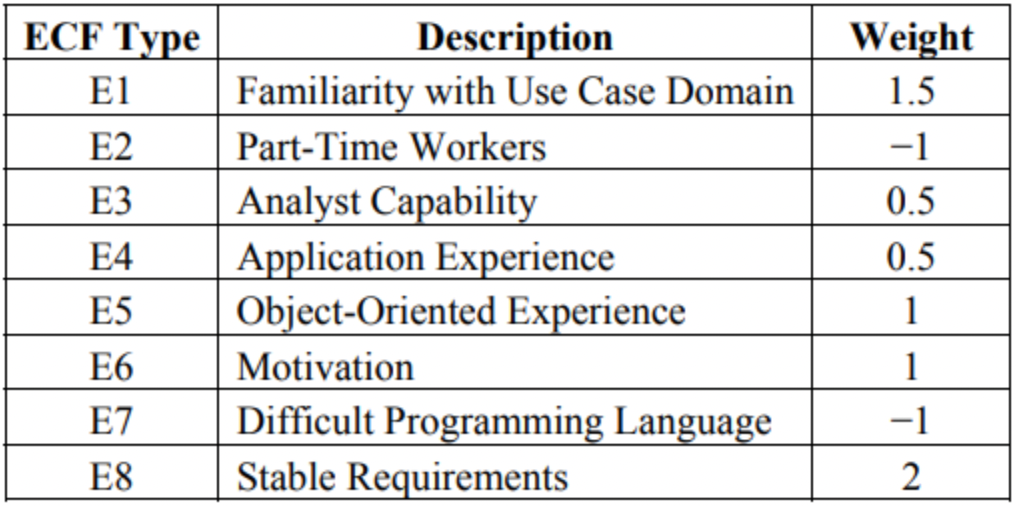
\includegraphics[width=14cm, height=6.01cm]{p8.png}
    \label{fig:Figure 8}
    \descriptionlabel{Table 2.1 The Environmental Complexity Factors in the UCP approach.}
\end{figure}


\normalsize{The equation is given by:}

\label{sec: Figure 9}
\begin{figure}[htp]
    \centering
    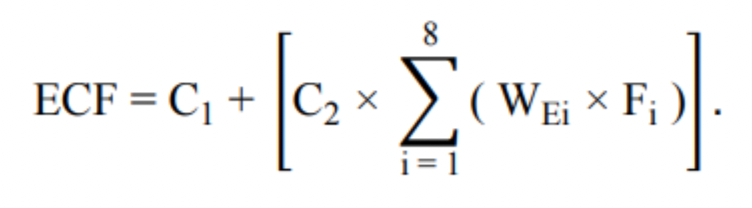
\includegraphics[width=8cm,height=2cm]{p9.png}
    \label{fig:Figure 9}
\end{figure}


\normalsize{C1=1.4 and C2=-0.03, WEi is ECF Weight, Fi is Perceived Impact Factor.\linebreak \\}

\normalsize{For Case: E1, E3, E4, E5, E6, and E8 -}
\begin{itemize}[noitemsep]
    \item 0-No influence
    \item 1-Strong,Negative influence
    \item 3-Average influence
    \item 5-Strong,Positive influence
\end{itemize}

\normalsize{For Case: E2 and E7-}
\begin{itemize}[noitemsep]
    \item 0-No influence
    \item 1-Strong Favourable influence
    \item 3-Average influence
    \item 5-Strong, Unfavourable influence.
\end{itemize}

\normalsize{From 2.5: }
\normalsize{ECF=1.4+(-0.03*((1.5*5)+(-1*0)+(0.5*3)+(0.5*3)+(1*5)+(1*5)+(-1*1)+(2*5)))\\}
\normalsize{ECF = 1.4−0.03(9+1.5+5+5−1+10)\\}
\normalsize{ECF = 1.4-0.03(29.5)\\}
\normalsize{ECF = 0.515 \linebreak \\}

\normalsize{From 2.2:\\}
\normalsize{UCP=UUCP*TCF*ECF\linebreak
UCP = 13*1.04*0.515\linebreak
UCP = 6.9628\linebreak}

\normalsize{From 2.1:\\}
\normalsize{Effort Estimate=UCP*PF\linebreak
Effort Estimate = 6.9628*20\linebreak
Effort Estimate = 139.25\linebreak}

\subsection{Using Basic COCOMO 81, provide an estimate of the effort towards the project.}

\normalsize{A method for estimating the amount of work needed to produce a software project based on the size of the software is the Basic COCOMO (Constructive Cost Model) 81.\linebreak}

\normalsize{E = a × $KLOC^{b}$\linebreak}

\normalsize{Let a = 2.4 and b = 1.05 as we are taking an estimate of an Organic Project. \linebreak
The estimate number of lines in the code is 500, so KLOC = 0.5 .\linebreak}

\normalsize{E = 2.4 × $(0.5)^{1.05}$ \linebreak
E = 1.15 PM(Person - Months)}

\normalsize{Now counting per hour effort,\linebreak
Hour-Effort = 1.15 * 22 * 4\linebreak
Hour-Effort = 102.002}


\subsection{Comment on the difference in estimates using the UCP approach and COCOMO 81, and the actual effort towards the project. 
}

\normalsize{Comment on the difference in estimates using the UCP approach and COCOMO 81, and the actual effort towards the project. \linebreak

\textbf{UCP Approach Estimate (139.25) Methodology:} UCP is a method for estimating software development effort based on the complexity and size of systems, considering factors like use cases and actors.\linebreak

\textbf{Calculation Process:} UCP involves determining Unadjusted Use Case Points (UUCP) by considering factors such as Technical Complexity Factor (TCF) and Environmental Complexity Factor (ECF).\linebreak

\textbf{Effort Estimation: }The estimated effort is obtained by multiplying UCP by the Productivity Factor (PF), resulting in a measure expressed in Person-Hours.\linebreak

\textbf{Specifics of Estimate (139.25 Person-Hours): }The UCP approach for the METRICSTICS application yielded an estimate of 139.25 Person-Hours, representing anticipated effort based on system characteristics, including user interactions and system complexity.\linebreak

\textbf{User Interaction and System Functionality: }UCP tends to consider user interactions and system functionality in detail, potentially leading to a higher estimated effort in certain cases.\linebreak

\textbf{Baseline for Comparison: }The UCP estimate serves as a baseline value for comparing different software estimation approaches.\linebreak


\textbf{COCOMO 81 Approach Estimate Methodology: }COCOMO 81 is a model for estimating software development effort based on project size (KLOC) and project type (Organic, Semi-Detached, or Embedded).\linebreak

\textbf{Calculation Process: }The COCOMO 81 approach involves estimating project size in Kilo Lines of Code (KLOC) and selecting the project type, with effort calculated using the Basic COCOMO 81 formula.\linebreak

\textbf{Effort Estimation: }The estimated effort, in the context of COCOMO 81, is determined by considering project size and complexity, resulting in a measure expressed in Person-Hours.\linebreak

\textbf{Specifics of Estimate (1.15 Person-Month): }The COCOMO 81 approach for the METRICSTICS application yielded an estimate of 1.15 Person-Month, representing anticipated effort based on project size and complexity.\linebreak

\textbf{Focus on Project Size and Complexity: }COCOMO 81 primarily focuses on project size and complexity as key factors influencing effort estimation.\linebreak

\textbf{Baseline for Comparison: }The COCOMO 81 estimate serves as a baseline value for comparing different software estimation approaches.\linebreak


\textbf{Estimate Difference: }The UCP approach, giving detailed consideration to user interactions and system functionality, projected a higher effort of 139.25 Person-Hours for the METRICSTICS application.\linebreak

Conversely, the COCOMO 81 approach, with its emphasis on project size and complexity, provided a lower estimate of 1.15 Person-Month.\linebreak

The substantial difference in estimates implies that the UCP approach encompassed additional factors or intricacies not addressed by the COCOMO 81 model in the specific context of the project.\linebreak
}
\subsection{Actual Project Effort:}
\normalsize{
\textbf{Real-Time Development Duration: }The METRICSTICS application was developed within a total timeframe of approximately 60-70 hours, a notable reduction compared to both UCP and COCOMO 81 estimates.\linebreak \\

\textbf{Factors Influencing Discrepancy: }Various factors contribute to this variance, including the efficiency of the development team, the adoption of contemporary development tools and practices, and a more focused project scope than initially envisioned in theoretical models.\linebreak \\ 

\textbf{Team Proficiency in Python: }The team's expertise in Python and familiarity with the utilized tools and libraries (such as Tkinter) played a significant role in streamlining development and reducing the actual time invested.
\linebreak \\
\textbf{Contributions of Effective Project Management: }Effective project management, clear requirements, and a streamlined development process further contributed significantly to minimizing the time and effort required for the project.
}


\newpage
\section{Problem 4: Implementation of Project METRICSTICS}

\normalsize{Python is a high-level, popular programming language in today’s world. It is known for readability and simplicity. Python syntax is also simple in fewer lines of code compared to other programming languages, making it an ideal choice for beginners. Another strength of Python is that it supports object-oriented programming.\linebreak} \\
\normalsize{Tkinter is Python’s standard GUI toolkit. Tkinter provides a wide range of tools and widgets to create interfaces for the application, including text box, button, menus, and other elements. Furthermore, Tkinter can be used on various operating systems, from MacOS, Windows to Linux. To make GUI simpler, Tkinter allows developers to customize the appearance of widgets using styles.  Below image depicts the usage of tkinter in our system}

\label{sec: Figure 10}
\begin{figure}[htp]
    \centering
    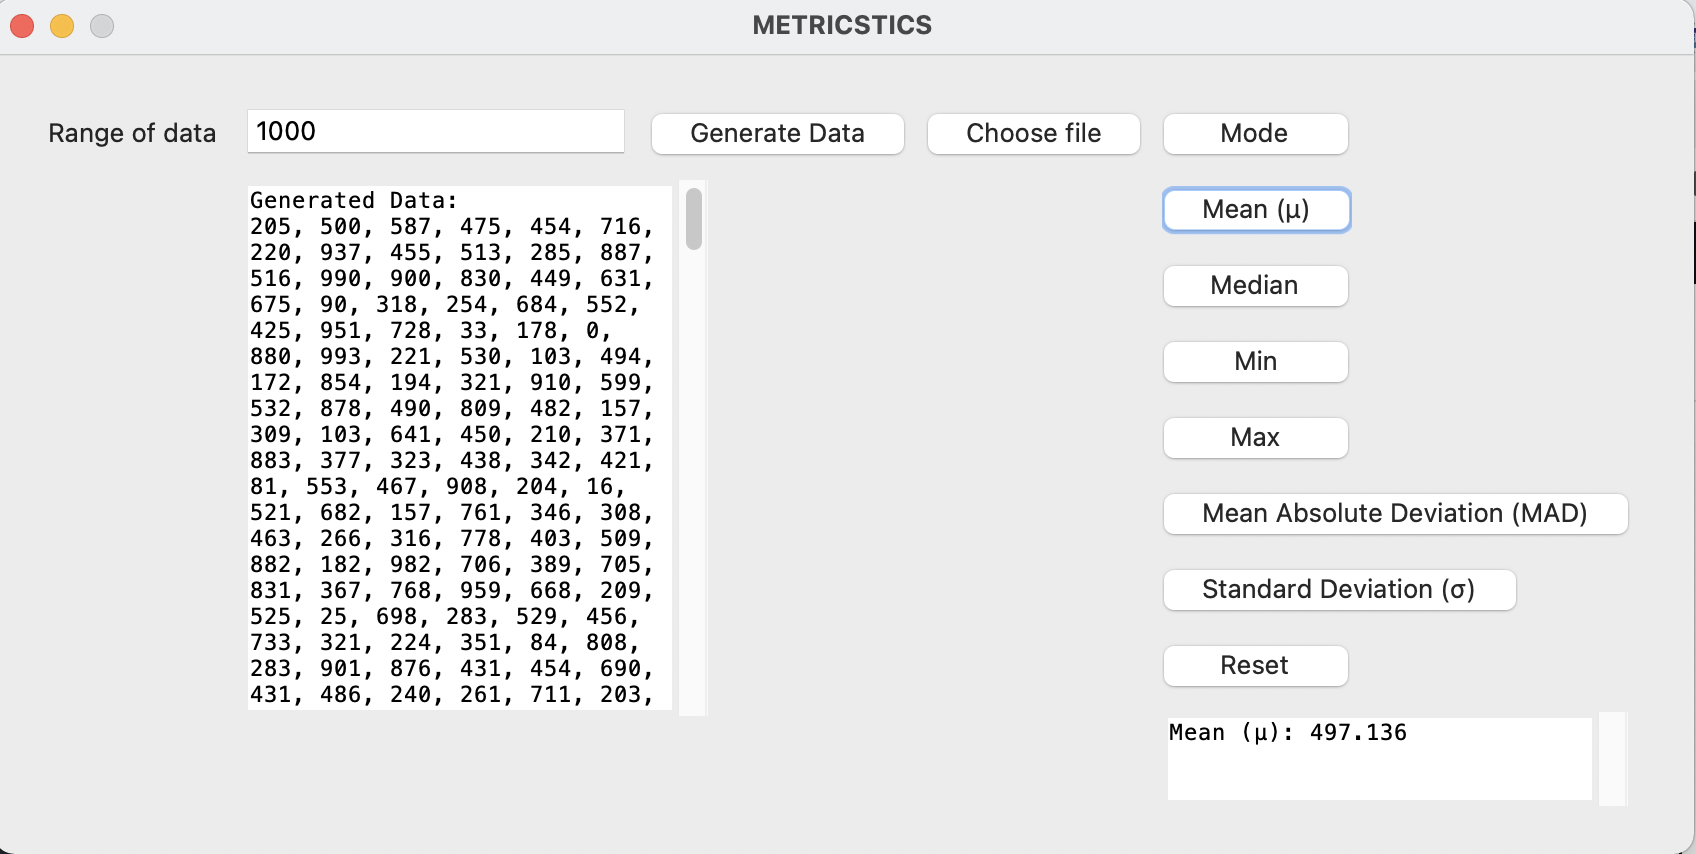
\includegraphics[width=16cm]{p10.png}
    \label{fig:Figure 10}
    \descriptionlabel{Fig 3.1 METRICSTICS Application}
\end{figure}

\pagebreak

\normalsize{GUI includes these components:}
\begin{itemize}[noitemsep]
    \item Range of data input: data that consists of (at least) 1000 values, randomly distributed between 0 and 1000. If users enter the wrong value, an error message will be displayed.
    \item "Generate data" button: press to generate sample data.
    \item "Choose file" button: press to upload an external file containing the dataset.
    \item Mode, Mean, Median, Min, Max, MAD, and Standard Deviation buttons.
    \item "Reset" button: reset all values in both result text and generated data text.
    \item Result text: display metric value from selection of users.
\end{itemize}

\label{sec: Figure 11}
\begin{figure}[htp]
    \centering
    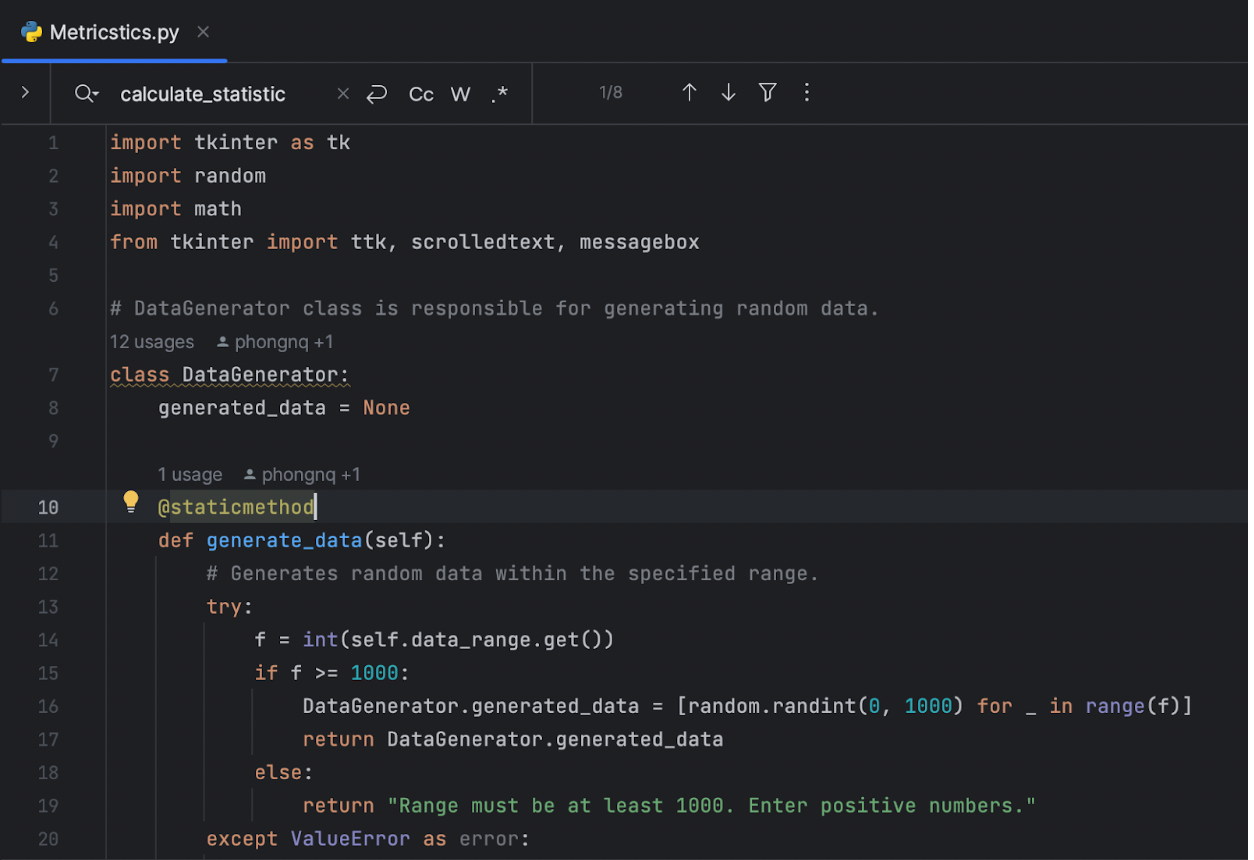
\includegraphics[width=15cm]{p11.png}
    \label{fig:Figure 11}
    \descriptionlabel{Fig 3.2 Code sample}
\end{figure}

\pagebreak

\label{sec: Figure 12}
\begin{figure}[htp]
    \centering
    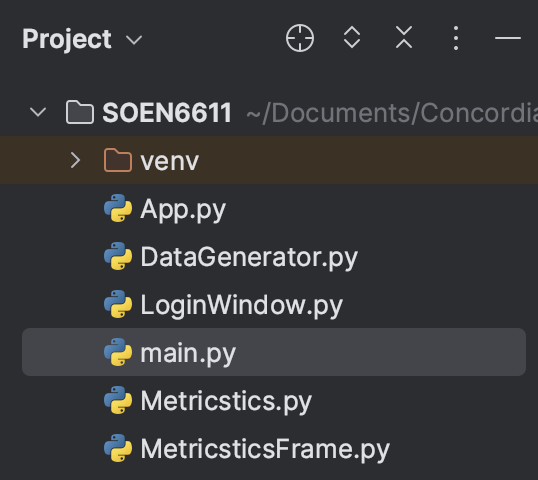
\includegraphics[width=12cm, height=10cm]{p12.png}
    \label{fig:Figure 12}
    \descriptionlabel{\\Fig 3.3 Class structure of METRICSTICS}
\end{figure}

\pagebreak


\section{Problem 5: Cyclomatic number}

\subsection{Cyclomatic number}

\subsection*{\textbf{Datagenarator.py}}

This file contains the \textbf{DataGenerator} class, which is responsible for generating random data. A static function, \textbf{generate\_data}, is included in the class. It receives a data range as input and generates random data within that range.

\subsection*{\textbf{Metrics.py}}

The \texttt{Metrics} class is included in the \texttt{Metrics.py} file and conducts numerous statistical calculations without the need for built-in functions. Minimum, maximum, mean, median, mode, mean absolute deviation, and standard deviation are all calculated.

\subsection*{\textbf{MetricsFrame.py}}

This file contains the \textbf{MetricsFrame} class, which is the application's main user interface. It generates data and performs statistical calculations using the \textbf{DataGenerator} and \textbf{Metrics} classes. Based on the tkinter library, the class contains methods for changing UI components and conducting calculations.

\subsection*{\textbf{LoginWindow.py}}

Represents a user login pop-up window in a tkinter-based Python application. Here, users are asked to enter credentials based on their role.

\subsection*{\textbf{App.py}}

This file defines the \textbf{App} class, which represents the primary application window. It extends the \textbf{tkinter.Tk} class and provides a \textbf{LoginWindow} class that handles user login. The \textbf{App} class handles the transition from the login screen to the main program window. This file also defines the application's entry point and primary event loop.
\linebreak


\normalsize{To obtain the cyclomatic complexity for each class and its corresponding values, I utilized a tool known as Radon from python library. This tool aids in analysing the complexity of software code by calculating the cyclomatic number, which provides valuable insights into the code’s structural intricacies and potential points of concern.\linebreak}\\

\normalsize{Here is the Cyclomatic number for each method in the provided Metristics.py:\linebreak}

\begin{itemize} 
    \item Metricstics:
   \begin{figure}[H]
    \centering
    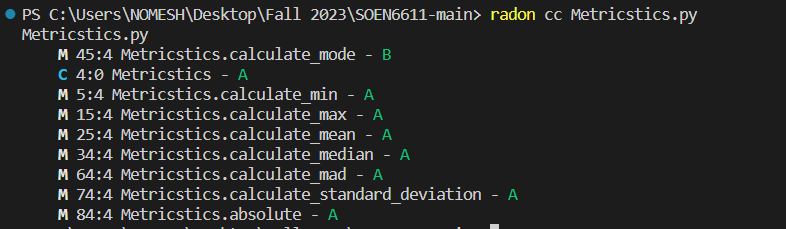
\includegraphics[width=1 \linewidth]{Metric_cc.png} 
    \descriptionlabel{Figure 4.1: Cyclometric complexity of Metricstics class}
\end{figure}
    \item MetricsticsFrame:
         \begin{figure}[H]
        \centering
        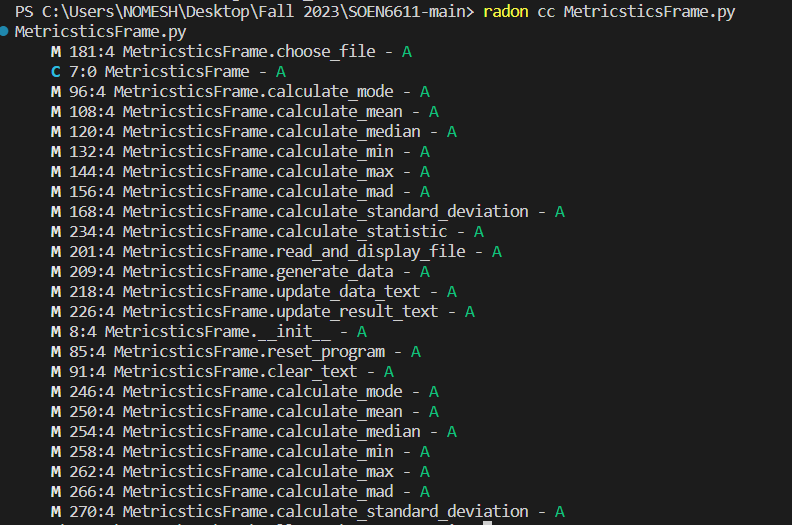
\includegraphics[width=1 \linewidth]{Metricstics_cc.png} 
        \descriptionlabel{Figure 4.2: Cyclometric complexity of MetricsticsFrame class}
        \linebreak \linebreak \linebreak
    \end{figure}
    \item DataGenerator:
         \begin{figure}[H]
        \centering
        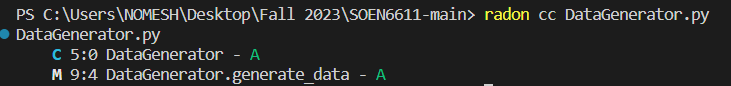
\includegraphics[width=1 \linewidth]{DataGenerator_cc.png} 
        \descriptionlabel{Figure 4.3: Cyclometric complexity of DataGenerator class}
    \end{figure}
    \item LoginWindow:
         \begin{figure}[H]
        \centering
        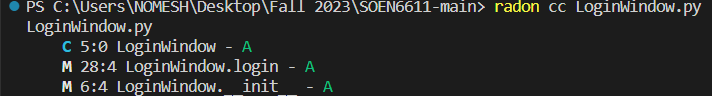
\includegraphics[width=1 \linewidth]{LoginWindow_cc.png} 
        \descriptionlabel{Figure 4.4: Cyclometric complexity of LoginWindow class}
    \end{figure}
        \end{itemize}
 
 \begin{itemize}
    \item App:
         \begin{figure}[H]
        \centering
        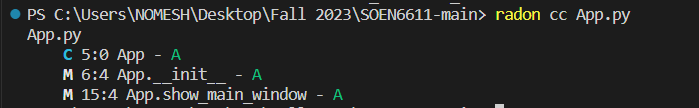
\includegraphics[width=1 \linewidth]{app_cc.png} 
        \descriptionlabel{Figure 4.5: Cyclometric complexity of App class}
    \end{figure}
        \end{itemize}

\normalsize{
Note: 
\begin{itemize}[noitemsep]
          \item   B indicates that the method contains decision points.
           \item  A indicates that the method does not contain decision points.
           \item  C indicates Class. 
           \item M indicates methods of the class.
            
            The Cyclomatic complexity is a measure of the complexity of a program. It is calculated based on the number of decision points in the control flow of the program. The higher the Cyclomatic complexity, the more complex the code is considered.
\end{itemize}

\pagebreak
\subsection{Conclusions for each classes:}

\textbf{\normalsize{LoginWindow Class:}}
\normalsize{Cyclomatic Complexity is moderately high. The cyclomatic complexity (1-2) is low, indicating a straightforward control flow at initialization.}

\textbf{\normalsize{App Class:}}
\normalsize{Overall, the App class has low Cyclomatic complexity, with simple and straightforward control flow in its \_\_init\_\_ method.\linebreak }

\textbf{\normalsize{MetricsticsFrame Class: }}
\normalsize{
\begin{itemize}[noitemsep]
    \item The MetricsticsFrame class exhibits a mix of Cyclomatic complexities.
    \item Several methods have low complexity (1-2), indicating simple control flow. 
    \item Some methods, such as calculate\_mode, calculate\_mean, etc., have moderate complexity (3-4), suggesting multiple decision points and branching paths. 
    \item Overall, the class has a varied level of control flow complexities. 
\end{itemize}}

\textbf{\normalsize{Metrics Class: }}
\normalsize{\begin{itemize}[noitemsep]
    \item The Metrics class contains methods related to statistical calculations.
    \item Several methods, like calculate\_mode and calculate\_mean, have moderate Cyclomatic complexity (3-7), indicating multiple decision points. 
    \item The complexity is generally moderate, reflecting the nature of statistical calculations. 
\end{itemize}}

\textbf{\normalsize{DataGenerator Class: }}
\normalsize{\begin{itemize}[noitemsep]
    \item The DataGenerator class, responsible for generating random data, has a moderate Cyclomatic complexity of 5 in its generate\_data method. 
    \item The complexity is associated with control flow during data generation. 
\end{itemize}}

\textbf{\normalsize{Summary: }}
\normalsize{\begin{itemize}[noitemsep]
    \item Each class has a mix of low to moderate Cyclomatic complexities, reflecting the diversity in the control flow within the methods. 
    \item Methods with simple control flow typically have a Cyclomatic complexity of 1-2. 
    \item Methods involving calculations or decision points have a moderate complexity (3-7). 
    \item Consideration for refactoring may be given to methods with higher complexities to enhance code maintainability. 
    \linebreak
\end{itemize}}



\newpage
\section{Problem 6: WMC, LF, LSOC }
\subsection{WMC: }
The Weighted Methods per Class (WMC) is calculated by obtaining the sum of the cyclomatic complexities for each method within a class. The non-normalized cyclomatic complexity values are used in this scenario. Therefore, the Weighted Methods per Class (WMC) for each class is as follows:

\begin{itemize}
  \item $WMC(\text{DataGenerator}) = 4$
  \item $WMC(\text{Metricstics}) = 33$
  \item $WMC(\text{MetricsticsFrame}) = 50$
  \item $WMC(\text{App}) = 4$
  \item $WMC(\text{LoginWindow}) = 7$
\end{itemize}

These values are calculated using the Radon library with the help of the following Python code.

\begin{verbatim}
import radon
from radon.complexity import cc_visit, sorted_results
import LoginWindow, Metricstics, MetricsticsFrame, App
import inspect

# Function to calculate WMC for a class
def calculate_wmc(class_instance):
    # Get class name
    class_name = class_instance.__name__

    # Get the code of the class
    class_code = inspect.getsource(class_instance)

    # Analyze the code and get the results
    results = cc_visit(class_code)
    complexities = [result.complexity for result in results]

    # Calculate WMC
    wmc = sum(complexities)

    return wmc

# Example usage:
my_class_instance = App
wmc_value = calculate_wmc(my_class_instance)
print("Weighted Method Per Class (WMC) for MyClass:", wmc_value)
\end{verbatim}

\normalsize{Where \textbf{myclassinstnace} will use Each class and generate WMC for that class}

\subsection{Comments of WMC: }
\begin{itemize}
    \item \textbf{DataGenerator:}
    \begin{itemize}
        \item $WMC(\text{DataGenerator}) = 4$
        \item The \texttt{DataGenerator} class has minimal complexity, indicating simple and linear control flow. It is easy to understand and maintain.
    \end{itemize}
    
    \item \textbf{Metricstics:}
    \begin{itemize}
        \item $WMC(\text{Metricstics}) = 33$
        \item The \texttt{Metricstics} class is somewhat complex, suggesting a fair number of decision points and control flow in its methods.
    \end{itemize}
    
    \item \textbf{MetricsticsFrame:}
    \begin{itemize}
        \item $WMC(\text{MetricsticsFrame}) = 50$
        \item The \texttt{MetricsticsFrame} class is more complicated, with methods involving more intricate control flow, decision points, and possibly nested structures.
    \end{itemize}
    
    \item \textbf{App:}
    \begin{itemize}
        \item $WMC(\text{App}) = 4$
        \item The \texttt{App} class has low complexity, indicating simple and linear control flow. It is easy to understand and maintain.
    \end{itemize}
    
    \item \textbf{LoginWindow:}
    \begin{itemize}
        \item $WMC(\text{LoginWindow}) = 7$
        \item The \texttt{LoginWindow} class has moderate complexity, suggesting methods with some decision points and control flow.
    \end{itemize}
\end{itemize}

Overall, the complexity levels vary among the classes. Some classes have low to moderate complexity (e.g., App, DataGenerator), while others (e.g., Metricstics, MetricsticsFrame) exhibit higher complexity.


\subsection{CF: }
The coupling factor (CF) [Abreu, 1995b; Harrison, Counsell, Nithi, 1998] measures the
average coupling between classes excluding coupling due to inheritance.\newline
Let C1, …, Cn be classes in an OOD, where n greater than 1.
Let IsClient(Ci, Cj) = 1, if class Ci has a relationship with class Cj; otherwise, it is 0. (In
other words, IsClient(Ci, Cj) is a characteristic function.)\newline
The semantics of the (is-client) relationship might be that an object of Ci calls a method
in Cj, or has a reference to Cj, or to an attribute in Cj. However, the requirement is that
this relationship cannot be inheritance. 

\begin{equation}
    CF = \frac{\sum_{i=1}^{n} \left( \sum_{j=1}^{n} \text{IsClient}(C_i, C_j) \right)}{n^2 - n}
\end{equation}
\newline
\normalsize{
\begin{itemize}
    \item App has dependencies on LoginWindow and MetricsticsFrame.
    \item Main has dependencies on App, Metricstics, and MetricsticsFrame.
    \item MetricsticsFrame has a dependency on DataGenerator.
\end{itemize}
\normalsize{here n=6 classes including main as a separate}
CF=(2+3+1+0+0+0)/($6^{2}$-6)\linebreak \linebreak
CF=6/30\linebreak \linebreak
CF = 0.20\linebreak \linebreak
The Coupling Factor is 0.20, indicating strong coupling among the classes. Each class has direct dependencies on the others, contributing to a higher coupling factor.
}

\subsection{LCOM: }

LCOM (Lack of Cohesion of Methods) is a metric used to measure the degree to which methods in a class are related to each other. It ranges from 0 to 1, where a lower value indicates better cohesion. The formula for LCOM is given by:

\[
LCOM = 1 - \frac{P}{Q}
\]

Where:

\begin{itemize}
    \item \(P\) is the number of disjoint sets of methods that do not share attributes.
    \item \(Q\) is the total number of method pairs in the class (excluding constructors and getters/setters).
\end{itemize}


 \subsection*{App Class: }
\begin{itemize}
    \item \textbf{Methods Using Similar Attributes:} show\_main\_window, init
    \item \textbf{Total Methods:} show\_main\_window, init, metrics\_calculator, login\_window
\end{itemize}

\textbf{LCOM Calculation:} $1 - \frac{P}{Q} = 1 - \frac{2}{6} = 0.67$

\subsection*{MetricsticsFrame Class: }
\begin{itemize}
    \item \textbf{Methods Using Similar Attributes:} calculate\_mode, calculate\_mean, calculate\_median, calculate\_min, calculate\_max, calculate\_mad, calculate\_standard\_deviation
    \item \textbf{Total Methods:} calculate\_mode, calculate\_mean, calculate\_median, calculate\_min, calculate\_max, calculate\_mad, calculate\_standard\_deviation, reset\_program, clear\_text, update\_data\_text, update\_result\_text
\end{itemize}

\textbf{LCOM Calculation:} $1 - \frac{P}{Q} = 1 - \frac{7}{66} = 0.89$

\subsection*{DataGenerator Class: }
\begin{itemize}
    \item \textbf{Methods Using Similar Attributes:} generate\_data
    \item \textbf{Total Methods:} generate\_data
\end{itemize}

\textbf{LCOM Calculation: } $1  - \frac{P}{Q} = 1 - \frac{0}{1} = 1$

\subsection*{Metricstics Class: }
\begin{itemize}
    \item \textbf{Methods Using Similar Attributes:} calculate\_min, calculate\_max, calculate\_mean, calculate\_median, calculate\_mode, calculate\_mad, calculate\_standard\_deviation, absolute
    \item \textbf{Total Methods:} calculate\_min, calculate\_max, calculate\_mean, calculate\_median, calculate\_mode, calculate\_mad, calculate\_standard\_deviation, absolute
\end{itemize}

\textbf{LCOM Calculation}} = $1  - \frac{P}{Q} = 1 - \frac{0}{28} = 1$ \linebreak

\subsection*{LoginWindow Class: }
\begin{itemize}
    \item \textbf{Methods Using Similar Attributes:} login
    \item \textbf{Total Methods:} login
    \linebreak
\end{itemize}

 \textbf{LCOM Calculation}} = $1  - \frac{P}{Q} = 1 - \frac{0}{1} = 1$ \linebreak \linebreak


\pagebreak
\textbf{\normalsize{Conclusion:  \\}}
\normalsize{
\begin{itemize}
\item \normalsize{ The App class exhibits moderate cohesion, suggesting that its methods are somewhat related.}
\item \normalsize{The MetricsticsFrame class shows moderate cohesion, indicating that its methods are somewhat related.}
\item \normalsize{The DataGenerator class demonstrates excellent cohesion with only one method and no disjoint sets.}
\item \normalsize{ The Metricstics class displays excellent cohesion, featuring multiple methods with no disjoint sets.}
\item \normalsize{The LoginWindow class exhibits excellent cohesion with only one method and no disjoint sets.}

\end{itemize}

\begin{figure}[htp]
    \centering
    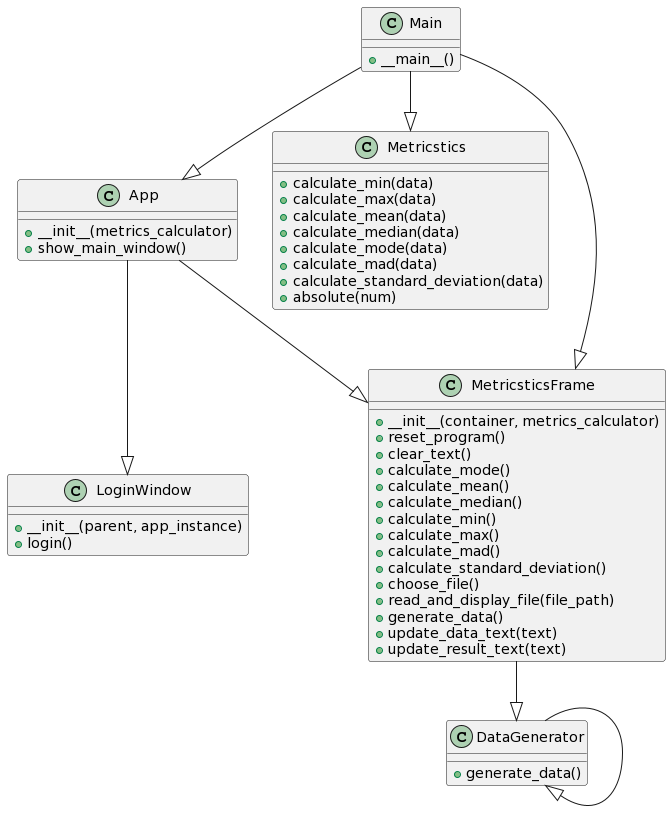
\includegraphics[width=16cm]{overalldepen.png}
    \descriptionlabel{Figure 5.1: Overall dependencies of the System}
\end{figure}

In summary, most of the classes exhibit high to excellent cohesion, suggesting that the methods within each class are well-organized and work effectively together. Overall, the codebase demonstrates good design principles with well-structured and cohesive classes. }

\pagebreak

\section{Problem 7: Physical And Logical SLOC }

\subsection{Goal: }
\normalsize{Goal Calculating the Physical SLOC and Logical SLOC for METRICSTICS. For Physical SLOC  and Logical SLOC a tool named Radon is used.}

\subsection{Physical SLOC: }
\normalsize{Physical SLOC refers to the count of lines in the source code containing executable statements, excluding blank lines and comments. In this project, the RADON tool was employed to calculate the Physical Source Lines of Code (Physical SLOC). \linebreak \\ 
RADON, a tool for performing static code analysis in Python, offers the capability to assess various code metrics, including Physical SLOC. The process involved utilizing RADON's functionalities to analyze the main directory. The tool provides insights into code complexity, maintainability, and other metrics. \linebreak \\
One advantage of using RADON is its suitability for Python projects, allowing for in-depth analysis and metrics calculation. By executing appropriate commands in the terminal or script, RADON aids in understanding the codebase's structure and complexity. \linebreak \\
In this specific project, the calculated Physical SLOC value of \textbf{445} lines indicates a smaller-sized system. This suggests lower complexity, making the codebase more manageable and easier to maintain due to its compact size. The utilization of RADON for code analysis aligns with the project's Python-centric nature, providing valuable metrics and facilitating informed decision-making in code maintenance and development. }

\subsection{Logical SLOC: }
\normalsize{It is a measure of the size or complexity of a software project based on the number of logical statements or instructions in the source code that affect the program’s control flow or behavior.\linebreak \\
Logical SLOC (Source Lines of Code) is a measure of the number of executable lines in code that contribute to the logical structure of the program. Here's a general guide on how logical SLOC is typically counted in Python code: \linebreak \\
\textbf{Advantages of Logical SLOC: }Measures essential code which indicates functionality, maintainability, and performance of the code \linebreak \\
Below fig represents the both Physical and Logical SLOC calculated using python:
}


\label{sec: Figure 5}
\begin{figure}[htp]
    \centering
    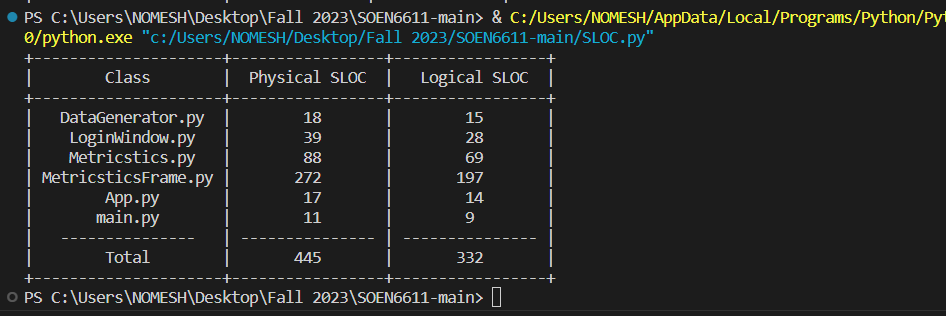
\includegraphics[width=15cm]{SLOC.png}
    \label{fig:Figure 5}
    \descriptionlabel{Figure 6.1: Physical and Logical SLOC}
\end{figure}

\normalsize{In summary, the logical SLOC count of 332 indicates a codebase of moderate size and complexity, which is likely to be well-structured and maintainable. It provides a foundation for further development and potential refactoring if necessary. }


\subsubsection{Rules for counting Physical SLOC and Logiccal SLOC}
\begin{table}[H]
    \centering
    \begin{tabular}{|p{3cm}|p{7cm}|p{5cm}|} \hline 
         Rule  &  Physical SLOC & Logical SLOC\\ \hline 
         
         Blank Lines  & Count each line that contains only spaces or tabs. & Ignore blank lines.  \\ \hline 
         
         Comment Lines  & Count each line that begins with a comment character (\#). & Ignore lines that contain only comments.\\ \hline 
         
         Executable Lines  & Count each line that contains executable code. & Count each line that contains executable code. \\ \hline 
         
         Multiline Strings  & Count each line inside triple-quoted strings (''' or """). & Ignore lines inside triple-quoted strings.  \\ \hline 
         Imports & Count each line with an import statement. & Ignore lines with import statements.  \\ \hline 
         Docstrings  & Count lines inside triple-quoted strings immediately after a class or function definition. & Ignore lines inside docstrings.  \\ \hline
         Empty Lines  & Count lines with no visible characters.  & Ignore lines with no visible characters. \\ \hline
         Logical Continuation  & Count each logical line as one line.  & Count each logical line as one line. \\ \hline
         Comments within Code  & Count comments embedded within code lines. & Ignore comments embedded within code lines. \\ \hline
         Single Line Comments & Count lines that contain a single-line comment. & Ignore lines that contain a single-line comment. \\ \hline
         Inline Comments & Count lines that have inline comments after executable code. & Ignore lines with inline comments. \\ \hline
    \end{tabular}
    \label{tab:my_label}
\end{table}
\pagebreak

\section{Problem 8}

    
\begin{table}[H]
    \RaggedRight
    \begin{tabular}{|c|c|c|} \hline
        Class & WMC & SLOC(L)  \\ \hline
        App & 4 & 14 \\ \hline
        DataGenerator & 4 & 15 \\ \hline
        LoginWindow & 7 & 28 \\ \hline
        MetristicsFrame & 33 & 69 \\ \hline
        Metristics & 50 & 197 \\ \hline
    \end{tabular}
    \label{tab:my_label}
\end{table}

\label{sec: Figure 13}
\begin{figure}[htp]
    \centering
    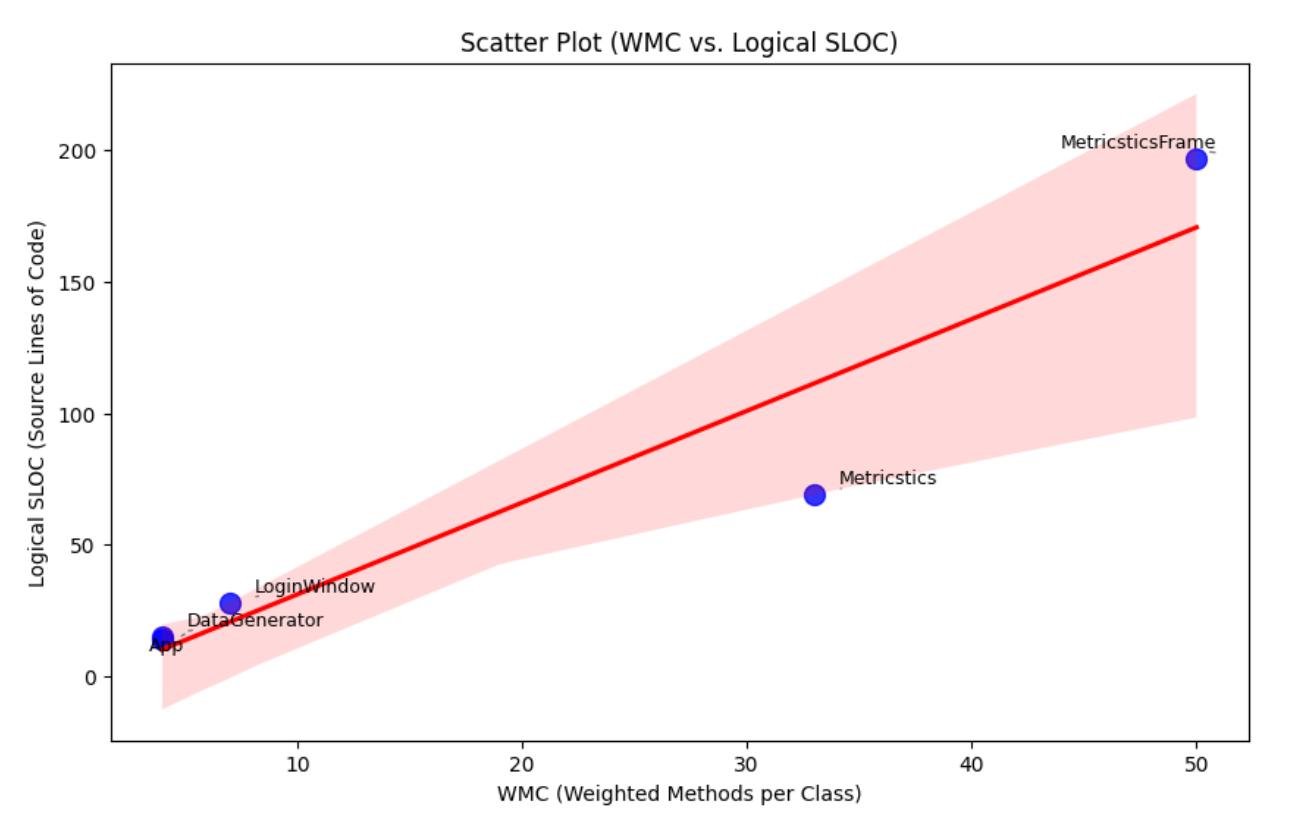
\includegraphics[width=16cm]{p13.png}
    \label{fig:Figure 13}
\end{figure}

\normalsize{We can see that there is a strong positive correlation between WMC and SLOC. This means that as the number of Weighted Methods in a Class (WMC) increases, the number of Source Lines of Code (SLOC) also tends to increase. This is likely because more complex classes tend to have more code.\linebreak \\
In the context of this problem, Spearman's rank correlation coefficient was used to measure the strength and direction of the association between Weighted Methods in a Class (WMC) and Source Lines of Code (SLOC). The coefficient was found to be 0.75, which indicates a strong positive correlation between the two variables. This means that as WMC increases, SLOC also tends to increase.\linebreak \\}
\normalsize{$\rho$ = 1 - (6 * $\Sigma d^{2})/(n(n^{2} - 1))$ \linebreak}

\begin{table}[H]
    \RaggedRight
\begin{tabular}{|c|c|c|c|c|c|c|} \hline
     & WMC & SLOC & Rank(WMC) & Rank(SLOC) & d & $d^{2}$ \\ \hline
    1 & 4 & 14 & 1.5 & 1 & 0.5 & 0.25 \\ \hline
    2 & 4 & 15 & 1.5 & 2 & -0.5 & 0.25 \\ \hline
    3 & 7 & 28 & 2 & 3 & -1 & 1 \\ \hline
    4 & 33 & 69 & 4 & 4 & -1 & 1 \\ \hline
    5 & 50 & 197 & 4 & 5 & -1 & 1 \\ \hline
\end{tabular}
\end{table}

\normalsize{$\Sigma d^{2}$ = 5\linebreak}
\normalsize{$\rho$ = 1 - (6*0.5)/(5*($5^{2}$ - 1)) = 0.9\linebreak}

\normalsize{The value of $\rho$ is 0.9, which indicates a strong positive correlation between WMC and SLOC. This means that the two variables are positively related, and that as WMC increases, SLOC also tends to increase.}

\pagebreak
\subsection*{Conclusion:}

\normalsize{The analysis of the correlations between the data for Logical SLOC and WMC obtained from METRICSTICS reveals a strong positive correlation between the two variables. As the number of Weighted Methods in a Class (WMC) increases, the number of Source Lines of Code (SLOC) also tends to increase. This finding aligns with the expectation that more complex classes, with a higher WMC, typically require more code to implement.\linebreak

The calculation of Spearman's rank correlation coefficient, a non-parametric measure of correlation, further confirms the existence of a strong positive correlation between WMC and SLOC. The coefficient value of 0.9 indicates a significant positive relationship between the two variables. This finding reinforces the notion that as WMC increases, SLOC also tends to increase.}

\vspace{\baselineskip}

\pagebreak

\section{Work Distribution}
\begin{table}[htb]
    \RaggedRight
    \begin{tabular}{|p{4cm}|p{5.5cm}|} \hline 
         Name & Contribution \\ \hline
         Quoc Phong Ngo [40230574] & Problem 4, developing the code and testing with various test cases \\ \hline
        SanVinoth Pacham [40198906] & Problem 4 \& 8, modifications and updates in the code, problem 8 \\ \hline
        Preet Angad Singh [40234930] & Problem 3 Use case point approach\\ \hline
        Siddharth Bharat Oza [40230155]	& Problem 3 COCOMO81 model, documentation of report in the latex\\ \hline
        Nomesh Palakaluri [40229979] & Problem 5,6,7 and documentation of the report\\ \hline
    \end{tabular}
    \label{tab:my_label}
\end{table}

\section{References}

\normalsize{\textit{tkinter — Python interface to Tcl/Tk: }}\\
\hyperlink{https://docs.python.org/3/library/tkinter.html}{https://docs.python.org/3/library/tkinter.html}
\newline
\newline
\normalsize{\textit{Developing a Full Tkinter Object-Oriented Application: }}\\
\hyperlink{https://www.pythontutorial.net/tkinter/tkinter-object-oriented-application/}{https://www.pythontutorial.net/tkinter/tkinter-object-oriented-application/}
\newline
\newline
\normalsize{\textit{Radon - Introduction to Code Metrics}}\\
\hyperlink{https://radon.readthedocs.io/en/latest/intro.html#cyclomatic-complexity}{https://radon.readthedocs.io/en/latest/intro.html#cyclomatic-complexity}
\newline
\newline
\normalsize{For genarating Palntuml code for class diagram based on our code}
\hyperlink{https://chat.openai.com/ }{https://chat.openai.com/ } 
\newline
\newline
\normalsize{Using the code genrated from chatgpt we plot dependency diagram}
\hyperlink{https://www.plantuml.com/plantuml/uml/SyfFKj2rKt3CoKnELR1Io4ZDoSa70000}{https://www.plantuml.com/plantuml/uml/SyfFKj2rKt3CoKnELR1Io4ZDoSa70000}



\vspace{\baselineskip}


\end{document}

